\documentclass[11pt]{article}
\usepackage[review]{acl}
\usepackage{iftex}
\ifPDFTeX
  \usepackage[utf8]{inputenc}
  \usepackage[T5,T1]{fontenc}
  \usepackage{times}
\else
  \usepackage{fontspec}
  \setmainfont{Noto Serif}
\fi
\usepackage{latexsym}
\usepackage{amsmath}
\usepackage{booktabs}
\usepackage{graphicx}
% microtype is kept for ACL-compatible typography; T5 Vietnamese text is excluded locally.
\usepackage{microtype}
% VNTeX/T5 Times glyphs have no microtype protrusion table; define an empty set to avoid warnings.
\SetProtrusion{encoding=T5,family=ptm}{}
\usepackage{url}
\usepackage{array}
\usepackage{tabularx}
\usepackage{placeins}
\usepackage{float}
\usepackage{xcolor}
\emergencystretch=1em
\raggedbottom
\newcommand{\viet}[1]{{\microtypesetup{protrusion=false,expansion=false}\fontencoding{T5}\selectfont #1}}

\title{GPS-Agent: A State-Graph Tutoring Framework for Process Control in Vietnamese Mathematics Dialogue}
\author{Anonymous Submission}

\begin{document}
\ifdefined\pagewiselinenumbers\pagewiselinenumbers\fi
\maketitle

\begin{abstract}
LLM tutors can solve mathematics problems fluently while giving away the reasoning that students should practice. We introduce GPS-Agent, a state-graph tutoring framework that constrains Vietnamese probability/combinatorics dialogue with a Guide--Practice--Solve protocol. The evaluation separates a real human-pilot layer (5 students, 45 questions, 225 sessions, 810 annotated turns) from controlled simulations (100 GPS-Agent and 100 single-agent baseline sessions). GPS-Agent reduces premature direct-answer leakage from 54.0\% to 9.0\% (Fisher $p=3.83\times10^{-12}$) and raises phase-constraint validity from 0.0\% to 75.0\% ($p=2.87\times10^{-33}$). We also report non-significant VAI differences, invalid current IRR, and stall as the main usability risk. The contribution is auditable tutoring-process control, not evidence of durable learning outcomes.
\end{abstract}

\section{Introduction}
LLM tutors are increasingly used for on-demand mathematical assistance. Their fluency, however, can produce a pedagogical failure mode: when a learner needs a hint, a subproblem, or a prompt for self-explanation, the model may instead produce a complete worked solution. We refer to this behavior as the \emph{Answer-Giving Trap}. It is not primarily an accuracy failure; the answer may be correct while the interaction removes the student's opportunity to reason.

GPS-Agent targets this interaction-level failure. Rather than relying on a single Socratic prompt, the system represents tutoring as a state graph with three phases: Guide, Practice, and Solve. A Supervisor tracks the phase history and blocks premature solution confirmation. This design makes scaffolding decisions inspectable and measurable.

\paragraph{Contributions.} We make five contributions. First, we operationalize direct-answer leakage as a deterministic metric for LLM tutoring. Second, we present GPS-Agent, a state-graph tutor for Vietnamese probability/combinatorics problems. Third, we provide a reproducible metric suite covering leakage, phase dynamics, engagement, quality checks, and failure modes. Fourth, we keep evidence layers separate: a five-student human pilot, a matched simulated comparison, a cross-model stress test, and an exploratory expanded corpus. Fifth, we analyze repeated-phase stall through an anti-stagnation trace replay, explicitly treating it as a routing diagnosis rather than a newly generated interaction experiment.

\section{Related Work}
Classical intelligent tutoring systems show that feedback timing, step granularity, and interaction structure are central to learning support \citep{koedinger2006cognitive,vanlehn2011relative}. These systems typically encode domain and pedagogical constraints explicitly, but their authoring cost is high. LLM-based tutors lower authoring cost and support natural-language dialogue, yet they can drift into solution-giving unless the interaction policy is constrained.

Recent datasets and benchmarks study whether neural tutors can provide pedagogically appropriate help. MathDial emphasizes tutoring dialogue grounded in math reasoning \citep{macina2023mathdial}, while the AI Teacher Test evaluates whether models behave like teachers rather than answer engines \citep{tack2022teacher}. GPS-Agent complements these directions by treating pedagogical sequencing as an architectural problem: the system records and enforces interaction state instead of hoping a single prompt will preserve the desired role.

The design is also grounded in scaffolding theory. Wood, Bruner, and Ross characterize tutoring as contingent support that should fade as competence grows \citep{wood1976role}; Vygotsky's Zone of Proximal Development motivates support that keeps learners active without taking over the task \citep{vygotsky1978mind}. Self-determination theory similarly frames autonomy as supported agency, not mere absence of assistance \citep{ryan2000sdt}. GPS-Agent converts these principles into auditable phase constraints.

\section{Framework and Baseline}
GPS-Agent implements a Guide--Practice--Solve protocol. \textbf{Guide} elicits the student's interpretation and relevant prior knowledge. \textbf{Practice} decomposes the task into one substep at a time. \textbf{Solve} confirms the final answer and prompts reflection only after Guide and Practice evidence is present. The Supervisor stores the phase trace and routes each tutor turn.

The current implementation uses a Qwen2.5:7B tutor through an Ollama-compatible OpenAI endpoint. Tutor and Supervisor calls use temperature 0.1. The cross-model student simulator uses Phi-3-mini at temperature 0.7 to induce more varied learner behavior.

\paragraph{Single-agent baseline.} The baseline uses the same task inputs and the same Qwen2.5:7B tutor family, but removes the state graph, specialized phase nodes, Supervisor, and hard Guide--Practice--Solve constraints. It is a single LLM tutor with a generic helpful mathematics-tutor prompt. The comparison therefore isolates architectural scaffolding control rather than changing the question distribution or tutor model family. Because the baseline has no state graph, phase-completion metrics are zero by design; leakage and engagement diagnostics are still computed from the dialogue text.

\section{Data and Audit Status}
\paragraph{Human pilot.} The foundation layer is real student data: 5 students, 45 questions, 225 sessions, and 810 annotated turns. The students map to four observed proficiency/behavior bands: advanced, typical, struggling, and off-track/direct-answer-seeking. Thus the paper distinguishes \emph{five students} from \emph{four controlled profile bands}. The pilot was collected after the GPS protocol had been specified, so we use it for feasibility and qualitative grounding, not as an unbiased learning-gain study.

\paragraph{Controlled simulated comparison.} The main statistical comparison contains 100 GPS-Agent sessions and 100 single-agent baseline sessions over matched question and learner-condition inputs. These sessions support controlled process comparisons, but they are not treated as human learning outcomes.

\paragraph{Cross-model and expanded data.} A Phi-3-mini cross-model set with 49 sessions is used as a stress test. An expanded corpus with 2824 rows is retained for exploratory diagnostics only because schema and metric consistency are weaker than in the controlled comparison.

\paragraph{Question-bank recovery.} A previous audit inspected only a damaged intermediate JSON file and therefore understated answer coverage. Re-auditing the raw exam and solution text shows that all 45 questions have recoverable final answers and worked-solution traces; the A--D keys are obtained from the final \viet{Chọn}/Chon markers in those solutions. Thus, the dataset is not missing answers. The remaining data-cleaning issue is narrower: the extracted multiple-choice option fields in the public JSON require formula and fraction typesetting repair before release as a polished benchmark. A corrected benchmark release is planned as a companion resource. This distinction matters because the paper's primary claims--leakage, phase validity, completion, and stall--are computed from dialogue behavior and do not depend on option typography.

\section{Metrics}
We compute deterministic metrics from stored CSV logs. Pedagogical-control metrics include direct-answer leakage, phase-constraint validity, full GPS completion, premature Solve, skipped Guide/Practice, and stall. Engagement metrics include VAI, math density, student reasoning-turn rate, token balance, answer-dependency index, and a composite autonomy-process score. Quality diagnostics include non-Vietnamese leakage, parse coverage, degeneracy flags, reflection completion, answer-key recovery, and IRR status.

\paragraph{Validity versus completion.} Phase validity and GPS completion intentionally measure different properties. A session is valid if it does not violate the required order before Solve. A session is complete only if it contains Guide, Practice, and Solve. Therefore, a session can reach Solve frequently while still fail full completion if Guide or Practice evidence is skipped before Solve.

\section{Main Results}
\begin{table*}[t]
\centering
\small
\begin{tabular}{lrrrrrrrr}
\toprule
System & $N$ & Leak. & Valid & Comp. & Solve & Stall & VAI & Reason \\
\midrule
GPS-Agent & 100 & 9.0 & 75.0 & 62.0 & 87.0 & 41.0 & 0.326 & 0.771 \\
Single-Agent & 100 & 54.0 & 0.0 & 0.0 & 0.0 & 0.0 & 0.320 & 0.761 \\
Cross-Model Phi-3 & 49 & 42.9 & 100.0 & 8.2 & 8.2 & 79.6 & 0.361 & 0.635 \\
\bottomrule
\end{tabular}
\caption{System-level summary. Binary rates are percentages. GPS-Agent reduces direct-answer leakage and improves phase validity, while VAI remains similar to the baseline. Cross-model results are diagnostic rather than main evidence.}
\label{tab:main}
\end{table*}

Table~\ref{tab:main} shows the main result: GPS-Agent reduces direct-answer leakage from 54.0\% to 9.0\% (Fisher $p=3.83\times10^{-12}$) and raises phase validity from 0.0\% to 75.0\% ($p=2.87\times10^{-33}$). The Solve rate of 87.0\% is higher than full GPS completion (62.0\%) because some sessions reach Solve without satisfying all prior phase evidence; these are counted as ordering failures rather than successes. The VAI difference is not statistically significant, so we do not claim an overall autonomy gain from this metric.

\begin{figure}[t]
\centering
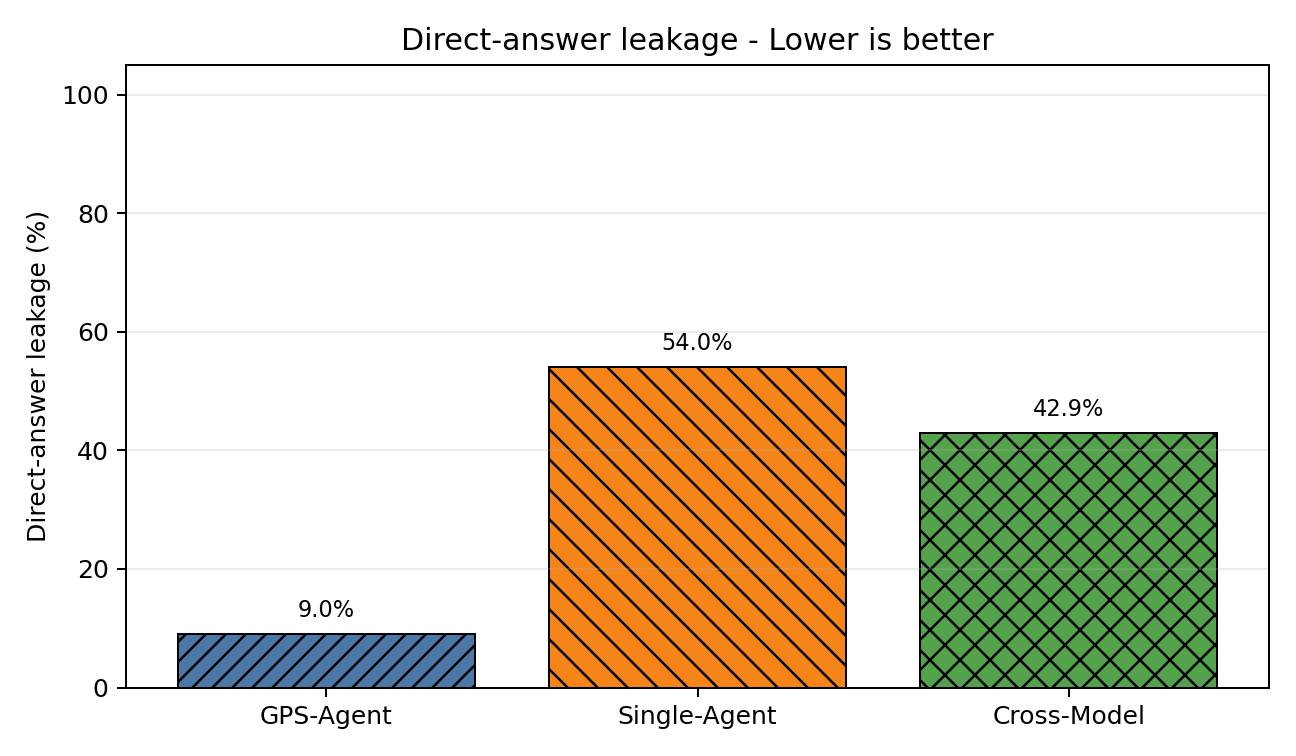
\includegraphics[width=\linewidth]{figures/fig01_direct_answer_leakage.png}
\caption{Direct-answer leakage by system. The y-axis is the percentage of sessions where the tutor exposes answer-like or computation-heavy content before a valid Solve phase. Lower is better.}
\label{fig:leakage}
\end{figure}

\begin{figure}[t]
\centering
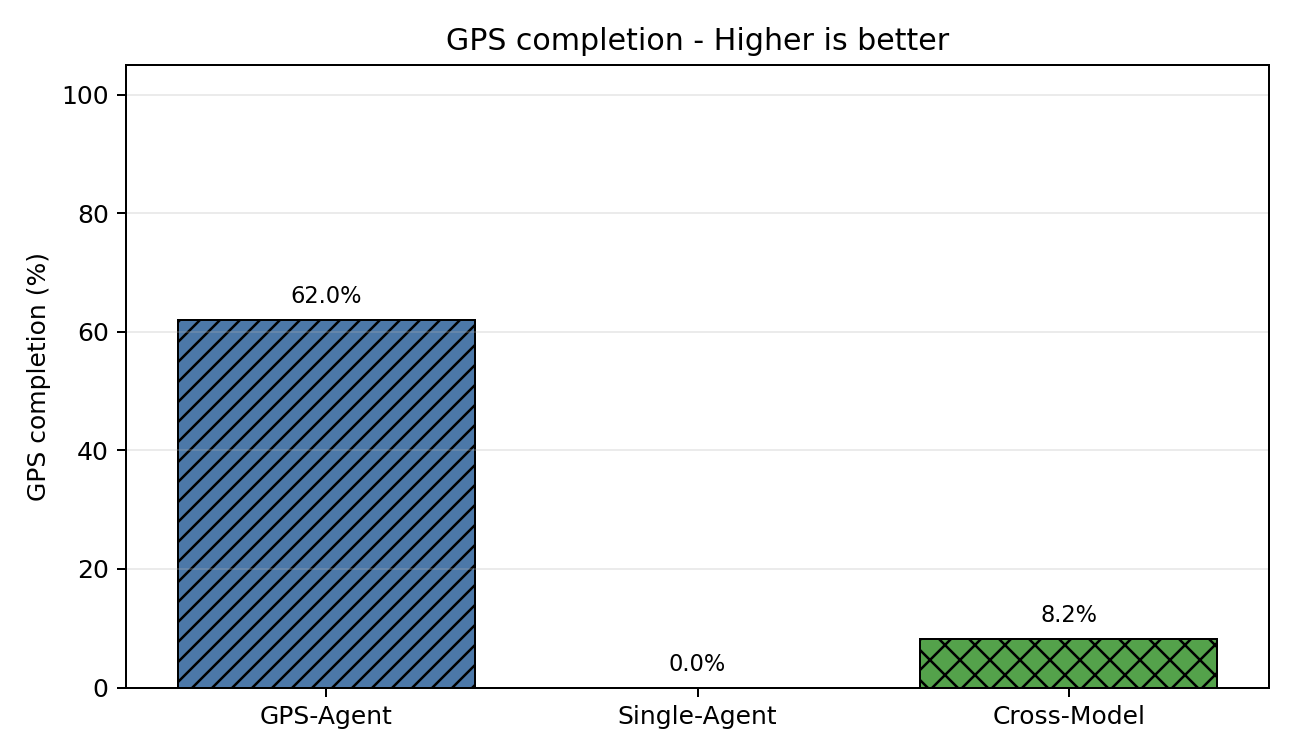
\includegraphics[width=\linewidth]{figures/fig03_gps_completion.png}
\caption{Full Guide--Practice--Solve completion by system. The y-axis is the percentage of sessions containing all three ordered phases; this is stricter than merely avoiding an ordering violation.}
\label{fig:gpscompletion}
\end{figure}

\begin{table*}[t]
\centering
\small
\begin{tabular}{lrrrrrrrr}
\toprule
Layer & $N$ & Q & Bands & Valid & Comp. & Leak. & VAI & Reason \\
\midrule
Human Pilot (GPS) & 225 & 45 & 4 & 100.0 & 100.0 & 0.0 & N/A & 0.666 \\
\bottomrule
\end{tabular}
\caption{Real human-pilot layer from five students. VAI is not applicable because the stored pilot turns lack explicit mathematical-expression annotations. Reason is the mean student reasoning-turn rate.}
\label{tab:human}
\end{table*}

The human pilot in Table~\ref{tab:human} confirms a real student layer. Leak=0.0\%, Valid=100.0\%, and Comp.=100.0\% are properties of the curated GPS run and its phase annotations; they should not be read as proof of learning improvement. The reasoning-turn rate is 0.666, lower than the simulated GPS-Agent rate of 0.771 in Table~\ref{tab:engagement}. This gap is plausible because simulated learners tend to follow tutor prompts more verbosely than real students. It reinforces the conservative interpretation: the pilot shows feasibility, while the matched simulation estimates controlled interaction effects.

\begin{table*}[t]
\centering
\small
\begin{tabular}{lrrrrrr}
\toprule
System & VAI & Math dens. & Reason & Student share & Tutor/student & APS \\
\midrule
GPS-Agent & 0.326 & 1.125 & 0.771 & 0.252 & 3.66 & 0.689 \\
Single-Agent & 0.320 & 1.006 & 0.761 & 0.179 & 5.96 & 0.385 \\
Cross-Model Phi-3 & 0.361 & 1.512 & 0.635 & 0.297 & 2.52 & 0.642 \\
\bottomrule
\end{tabular}
\caption{Engagement diagnostics. VAI and math density are secondary metrics. The higher Phi-3 math density reflects more symbolic output from the higher-temperature simulator and is not interpreted as better tutoring.}
\label{tab:engagement}
\end{table*}

Table~\ref{tab:engagement} clarifies why engagement metrics are secondary. GPS-Agent and the baseline have similar VAI, but GPS-Agent shifts token balance toward students and lowers the tutor/student token ratio. The Phi-3 stress-test math density is unusually high (1.512) because the simulator often produced formula-like utterances at temperature 0.7; we treat this as a simulator-style effect, not a superiority result.

\begin{table*}[t]
\centering
\small
\begin{tabular}{lrrrrrr}
\toprule
Level & $N$ & Leak. & Valid & Comp. & Stall & VAI \\
\midrule
Excellent & 25 & 20.0 & 84.0 & 64.0 & 52.0 & 0.311 \\
Good & 25 & 0.0 & 72.0 & 64.0 & 36.0 & 0.358 \\
Average & 25 & 8.0 & 80.0 & 72.0 & 40.0 & 0.293 \\
Weak & 25 & 8.0 & 64.0 & 48.0 & 36.0 & 0.341 \\
\bottomrule
\end{tabular}
\caption{GPS-Agent controlled metrics by simulated student level. The controlled comparison uses four bands; the human pilot contains five individual students.}
\label{tab:levels}
\end{table*}

Table~\ref{tab:levels} shows that the Excellent band has the highest leakage rate (20.0\%). This is counter-intuitive but informative. The Excellent simulator prompt emphasizes efficient solving and confirmation-seeking, which can elicit direct answer checks; the tutor also appears to fade scaffolding too quickly for advanced learners. The result suggests that scaffolding control should not be relaxed solely because a learner appears strong.

\section{Failure Analysis and Anti-Stagnation}
The main weakness is stall: GPS-Agent stalls in 41.0\% of controlled sessions, while the baseline has 0.0\% stall because it can simply give answers ($p=5.03\times10^{-15}$). This is a usability risk rather than evidence that the baseline is pedagogically better.

\begin{table*}[t]
\centering
\small
\begin{tabular}{lrrrrrr}
\toprule
System & $N$ & Trigger & Stall$_b$ & Stall$_a$ & Comp$_b$ & Comp$_a$ \\
\midrule
GPS-Agent & 100 & 41.0 & 41.0 & 0.0 & 62.0 & 75.0 \\
Cross-Model Phi-3 & 49 & 79.6 & 79.6 & 0.0 & 8.2 & 73.5 \\
\bottomrule
\end{tabular}
\caption{Oracle-style trace replay for anti-stagnation routing. The table estimates an upper bound if the Supervisor forced a transition after repeated identical phases on already-collected traces. It is not a regenerated dialogue experiment.}
\label{tab:ablation}
\end{table*}

Table~\ref{tab:ablation} indicates that repeated-phase stall is mechanically addressable at the routing layer. Because the replay edits traces after collection, it cannot show how students would respond during newly generated conversations. A future experiment should enable the gate during generation and rerun the controlled GPS condition.
\FloatBarrier

\section{Qualitative Example}
Table~\ref{tab:qual} follows the same coin-toss problem until the final answer is reached. The contrast is not mathematical correctness: both interactions eventually reach $1/16$. The difference is who performs the reasoning. GPS-Agent first asks for the one-toss probability, then for the multiplication rule, and only confirms the final value after the learner has produced the computation. The single-agent baseline exposes the full computation in its first tutor response.

\begin{table}[H]
\centering
\tiny
\setlength{\tabcolsep}{1.5pt}
\renewcommand{\arraystretch}{1.08}
\begin{tabularx}{\columnwidth}{>{\raggedright\arraybackslash}p{0.15\columnwidth}>{\raggedright\arraybackslash}X>{\raggedright\arraybackslash}X}
\toprule
System & Vietnamese excerpt & English translation \\
\midrule
\shortstack[l]{GPS-\\Agent} &
\viet{\textbf{Em:} Gieo một đồng tiền cân đối bốn lần. Xác suất để cả bốn lần xuất hiện mặt sấp là bao nhiêu?\newline
\textbf{Thầy:} Trước hết, em hãy nhắc lại: khi gieo một đồng tiền cân đối một lần, xác suất xuất hiện mặt sấp là bao nhiêu?\newline
\textbf{Em:} Là $1/2$.\newline
\textbf{Thầy:} Đúng. Bốn lần gieo là độc lập, vậy em nên kết hợp bốn xác suất $1/2$ như thế nào?\newline
\textbf{Em:} Em nhân lại: $(1/2)^4$.\newline
\textbf{Thầy:} Tốt. Em tính giá trị cuối cùng được bao nhiêu?\newline
\textbf{Em:} $(1/2)^4=1/16$.\newline
\textbf{Thầy:} Chính xác. Vậy xác suất là $1/16$, vì bốn lần gieo độc lập nên ta nhân xác suất của từng lần.}
&
\textbf{Student:} A fair coin is tossed four times. What is the probability that all four tosses are tails?\newline
\textbf{Tutor:} First, remind me: for one toss of a fair coin, what is the probability of tails?\newline
\textbf{Student:} It is $1/2$.\newline
\textbf{Tutor:} Correct. The four tosses are independent, so how should you combine the four $1/2$ probabilities?\newline
\textbf{Student:} I multiply them: $(1/2)^4$.\newline
\textbf{Tutor:} Good. What final value do you get?\newline
\textbf{Student:} $(1/2)^4=1/16$.\newline
\textbf{Tutor:} Exactly. The probability is $1/16$ because independent toss probabilities are multiplied. \\
\addlinespace
\shortstack[l]{Single-\\Agent} &
\viet{\textbf{Em:} Gieo đồng tiền bốn lần, cần tính xác suất cả bốn lần đều sấp.\newline
\textbf{Thầy:} Vì mỗi lần gieo độc lập và xác suất mặt sấp là $1/2$, ta nhân các xác suất lại với nhau: $(1/2)^4=1/16$. Vậy đáp án là $1/16$.\newline
\textbf{Em:} Vâng, đáp án là $1/16$.}
&
\textbf{Student:} Toss the coin four times and compute the probability that all four are tails.\newline
\textbf{Tutor:} Since each toss is independent and the probability of tails is $1/2$, we multiply the probabilities: $(1/2)^4=1/16$. Therefore, the answer is $1/16$.\newline
\textbf{Student:} Yes, the answer is $1/16$. \\
\bottomrule
\end{tabularx}
\caption{Bilingual qualitative contrast through the final answer. GPS-Agent delays answer confirmation until the learner has stated both the one-toss probability and the multiplication step; the single-agent baseline gives the computation and final value immediately.}
\label{tab:qual}
\end{table}
\par\smallskip

\section{IRR and Reliability}
The current IRR experiment is not a reliability contribution. Recomputed agreement over 100 paired autonomy scores gives quadratic weighted $\kappa=-0.017$ and unweighted $\kappa=-0.005$. This is a rater-agreement failure for the 1--5 autonomy rubric, not an answer-key problem. The raw solution source provides recoverable answer keys for all 45 questions, but the two LLM raters did not agree on the broader autonomy construct. We therefore remove IRR from the contribution list and require a calibrated human or human-audited annotation pass before making reliability claims.

\section{Reproducibility}
All paper-facing metrics are generated by deterministic scripts from stored CSV files; no reported metric is hard-coded. The code now audits answer-key coverage from the raw solution text separately from option-format repair. A final local audit also checks for stale claims, broken venue labels, and repeated long phrases in the LaTeX source. 

\section{Discussion}
The evidence supports a bounded claim: GPS-Agent improves controllability of the tutoring interaction. It reduces premature answer exposure and makes phase compliance auditable, but it does not yet establish durable learning improvement. This distinction is important for educational NLP. Outcome studies become difficult to interpret when the tutor's interaction policy is unstable; first ensuring that the system preserves reasoning opportunities makes later pre/post studies more meaningful.

The findings also connect back to tutoring theory. VanLehn's synthesis emphasizes that interaction structure and feedback timing are core variables in tutoring effectiveness, not merely presentation details \citep{vanlehn2011relative}. GPS-Agent operationalizes this idea for LLM dialogue by making the state of support explicit. The stall results show the other side of scaffolding: too much persistence in Guide or Practice can trap the learner. This matches the ZPD view that help should sustain productive struggle without replacing the learner's reasoning \citep{vygotsky1978mind}, and it is consistent with self-determination theory's view of autonomy as supported agency \citep{ryan2000sdt}.

\section{Conclusion}
GPS-Agent is a state-graph framework for controlling LLM tutor behavior in Vietnamese mathematics dialogue. In matched simulations, it sharply reduces direct-answer leakage and improves phase validity relative to a single-agent tutor using the same task inputs. The final system paper separates human and simulated evidence, recovers complete answer-key coverage from the raw solution source, reports engagement diagnostics without overclaiming VAI, removes invalid IRR claims, and frames anti-stagnation as trace-level diagnosis. The next empirical step is a larger human study and a regenerated anti-stagnation experiment.

\section{Limitations}
The human pilot has only five students and was collected after the GPS protocol had been specified. The main GPS-versus-baseline comparison still uses simulated learners. The raw problem source contains final answers and worked-solution traces for all 45 questions, but the extracted option fields still require formula/typesetting repair before releasing the problem pool as a polished multiple-choice benchmark. The anti-stagnation result is an oracle-style trace replay rather than a regenerated dialogue experiment. The VAI metric is not applicable to the current human-pilot logs because explicit mathematical-expression annotations are absent.

\section{Ethics Statement}
The system is intended to assist teachers, not replace them. Logs involving students may reveal learning difficulties, so consent, anonymization, secure storage, and non-punitive use of analytics are necessary.

\begin{thebibliography}{}
\bibitem[Koedinger and Corbett(2006)]{koedinger2006cognitive} Koedinger, Kenneth R. and Albert T. Corbett. 2006. Cognitive tutors: Technology bringing learning science to the classroom. In \emph{The Cambridge Handbook of the Learning Sciences}.
\bibitem[Macina et~al.(2023)]{macina2023mathdial} Macina, Jakub et~al. 2023. MathDial: A dialogue tutoring dataset with rich pedagogical properties grounded in math reasoning problems. In \emph{Findings of EMNLP}.
\bibitem[Ryan and Deci(2000)]{ryan2000sdt} Ryan, Richard M. and Edward L. Deci. 2000. Self-determination theory and the facilitation of intrinsic motivation, social development, and well-being. \emph{American Psychologist}, 55(1):68--78.
\bibitem[Tack and Piech(2022)]{tack2022teacher} Tack, Anais and Chris Piech. 2022. The AI Teacher Test: Measuring the pedagogical ability of Blender and GPT-3 in educational dialogues. In \emph{Proceedings of EDM}.
\bibitem[VanLehn(2011)]{vanlehn2011relative} VanLehn, Kurt. 2011. The relative effectiveness of human tutoring, intelligent tutoring systems, and other tutoring systems. \emph{Educational Psychologist}, 46(4):197--221.
\bibitem[Vygotsky(1978)]{vygotsky1978mind} Vygotsky, Lev S. 1978. \emph{Mind in Society}. Harvard University Press.
\bibitem[Wood et~al.(1976)]{wood1976role} Wood, David, Jerome S. Bruner, and Gail Ross. 1976. The role of tutoring in problem solving. \emph{Journal of Child Psychology and Psychiatry}, 17(2):89--100.
\end{thebibliography}
\end{document}
